\documentclass[a4paper]{scrartcl}

\usepackage[
    fancytheorems, 
    fancyproofs, 
    noindent, 
]{adam}


\title{Geometry}
\author{Adam Kelly (\texttt{ak2316@cam.ac.uk})}
\date{\today}

\allowdisplaybreaks

\begin{document}

\maketitle

% This is a short description of the course. It should give a little flavour of what the course is about, and what will be roughly covered in the notes.

This article constitutes my notes for the `Non-Existent' course, held in Lent 2022 at Cambridge. These notes are \emph{not a transcription of the lectures}, and differ significantly in quite a few areas. Still, all lectured material should be covered.



\tableofcontents

\section{Topological and Smooth Surfaces}

\subsection{Topological Surfaces}


It is not to hard to think up many exotic 'surfaces' with different characteristics: holes, no holes, bounded, unbounded, and so on.

\begin{center}
    

\tikzset{every picture/.style={line width=0.75pt}} %set default line width to 0.75pt        

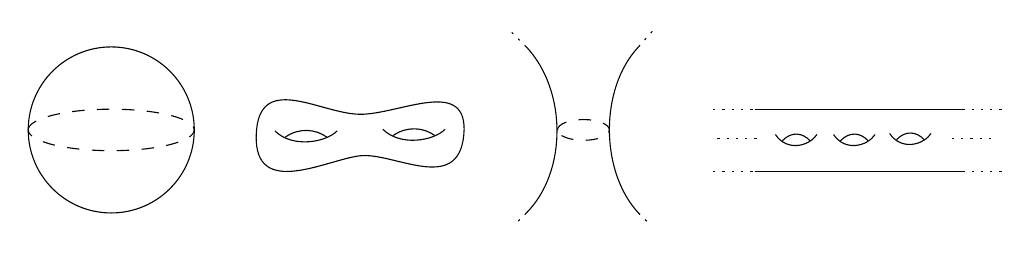
\begin{tikzpicture}[x=0.75pt,y=0.75pt,yscale=-1,xscale=1]
%uncomment if require: \path (0,300); %set diagram left start at 0, and has height of 300

%Shape: Circle [id:dp591684684256957] 
\draw   (60,110) .. controls (60,87.91) and (77.91,70) .. (100,70) .. controls (122.09,70) and (140,87.91) .. (140,110) .. controls (140,132.09) and (122.09,150) .. (100,150) .. controls (77.91,150) and (60,132.09) .. (60,110) -- cycle ;
%Shape: Ellipse [id:dp6271436208495527] 
\draw  [dash pattern={on 4.5pt off 4.5pt}] (60,110) .. controls (60,104.48) and (77.91,100) .. (100,100) .. controls (122.09,100) and (140,104.48) .. (140,110) .. controls (140,115.52) and (122.09,120) .. (100,120) .. controls (77.91,120) and (60,115.52) .. (60,110) -- cycle ;
%Shape: Polygon Curved [id:ds2919643672856125] 
\draw   (169.85,112.46) .. controls (170.85,81.46) and (200.85,102.32) .. (219.85,102.46) .. controls (238.85,102.6) and (272.56,83.74) .. (269.85,112.46) .. controls (267.13,141.17) and (235.99,120.6) .. (219.85,122.46) .. controls (203.7,124.32) and (168.85,143.46) .. (169.85,112.46) -- cycle ;
%Curve Lines [id:da29495862583968235] 
\draw    (178.85,110.46) .. controls (187.18,118.79) and (203.18,116.13) .. (208.85,110.46) ;
%Curve Lines [id:da05574670652938796] 
\draw    (183.85,113.46) .. controls (190.56,108.74) and (198.56,109.6) .. (203.85,113.46) ;
%Curve Lines [id:da9130401683536076] 
\draw    (230.85,109.68) .. controls (239.18,118.01) and (255.18,115.35) .. (260.85,109.68) ;
%Curve Lines [id:da7204510994314768] 
\draw    (235.85,112.68) .. controls (242.56,107.97) and (250.56,108.82) .. (255.85,112.68) ;
%Curve Lines [id:da2773823088001599] 
\draw    (300,70) .. controls (319.67,91) and (319.67,130.33) .. (300,150) ;
%Curve Lines [id:da9640418131331623] 
\draw    (354,70) .. controls (335,90.33) and (335.67,130.33) .. (354,150) ;
%Shape: Ellipse [id:dp22219783359667034] 
\draw  [dash pattern={on 4.5pt off 4.5pt}] (315,110) .. controls (315,107.24) and (320.6,105) .. (327.5,105) .. controls (334.4,105) and (340,107.24) .. (340,110) .. controls (340,112.76) and (334.4,115) .. (327.5,115) .. controls (320.6,115) and (315,112.76) .. (315,110) -- cycle ;
%Straight Lines [id:da16456755952599722] 
\draw  [dash pattern={on 0.84pt off 2.51pt}]  (354,70) -- (362,61) ;
%Straight Lines [id:da7546245438033814] 
\draw  [dash pattern={on 0.84pt off 2.51pt}]  (300,70) -- (293,63) ;
%Straight Lines [id:da9016788212880511] 
\draw  [dash pattern={on 0.84pt off 2.51pt}]  (300,150) -- (294,156) ;
%Straight Lines [id:da09916176203257931] 
\draw  [dash pattern={on 0.84pt off 2.51pt}]  (354,150) -- (360,156) ;
%Straight Lines [id:da28760276070953084] 
\draw    (410,100) -- (510,100) ;
%Straight Lines [id:da6331102333453389] 
\draw  [dash pattern={on 0.84pt off 2.51pt}]  (510,100) -- (530,100) ;
%Straight Lines [id:da21402696096677087] 
\draw  [dash pattern={on 0.84pt off 2.51pt}]  (390,100) -- (410,100) ;
%Straight Lines [id:da1318444055095227] 
\draw    (410,130) -- (510,130) ;
%Straight Lines [id:da3814972937738479] 
\draw  [dash pattern={on 0.84pt off 2.51pt}]  (510,130) -- (530,130) ;
%Straight Lines [id:da5990977106686659] 
\draw  [dash pattern={on 0.84pt off 2.51pt}]  (390,130) -- (410,130) ;
%Curve Lines [id:da8167058041805688] 
\draw    (420,112.22) .. controls (425.56,120.56) and (436.22,117.89) .. (440,112.22) ;
%Curve Lines [id:da07278542081013839] 
\draw    (423.33,115.22) .. controls (427.81,110.51) and (433.14,111.37) .. (436.67,115.22) ;
%Curve Lines [id:da23375889947741713] 
\draw    (448,112.22) .. controls (453.56,120.56) and (464.22,117.89) .. (468,112.22) ;
%Curve Lines [id:da8125417949179057] 
\draw    (451.33,115.22) .. controls (455.81,110.51) and (461.14,111.37) .. (464.67,115.22) ;
%Curve Lines [id:da989215927108835] 
\draw    (475,111.7) .. controls (480.56,120.04) and (491.22,117.37) .. (495,111.7) ;
%Curve Lines [id:da7272978688417131] 
\draw    (478.33,114.7) .. controls (482.81,109.99) and (488.14,110.85) .. (491.67,114.7) ;
%Straight Lines [id:da2512282339351666] 
\draw  [dash pattern={on 0.84pt off 2.51pt}]  (505,114) -- (525,114) ;
%Straight Lines [id:da05590955730268288] 
\draw  [dash pattern={on 0.84pt off 2.51pt}]  (392,114) -- (412,114) ;




\end{tikzpicture}

\end{center}

In this course we will frequently deal with such surfaces, and they are studied through the lense of topological surfaces.

\begin{definition}[Topological Surface]
    A topological surface is a topological space $\Sigma$ such that
    \begin{enumerate}[label=(\roman*)]
        \item Each $p \in \Sigma$ has an open neighbourhood $U$ with $p \in U$ such that $U$ is homeomorphic to $\R^2$, with its usual Euclidean topology.
        \item $\Sigma$ is Hausdorff and second countable.
    \end{enumerate}    
\end{definition}



% We care a significant amount about $X$ random object.

% \begin{definition}[Random Object]
%     We say that an object $X$ is a \vocab{random object} if we literally do not care about what it actually is.
% \end{definition}

% It is trivial to check that all objects you will meet in this course are random objects.


\end{document}
